\section{Experiments}
\label{sec:exp}
\paragraph{Datasets.} Our study illustrates the adaptability of {\ours} in dynamically managing the trade-off between computation and performance based on M2F \cite{cheng2021mask2former} meta-architecture. We do this on two widely used image segmentation datasets: COCO \cite{lin2014microsoft} and Cityscapes \cite{cordts2016cityscapes}. COCO comprises 80 ``things'' and 53 ``stuff'' categories, with 118k training images and 5k validation images. Cityscapes consists of 8 ``things'' and 11 ``stuff'' categories, with approximately 3k training images and 500 validation images. The evaluation is conducted over the union of ``things'' and ``stuff'' categories.

\paragraph{Evaluation metrics.}
We follow the evaluation setting of \cite{cheng2021mask2former} for evaluation of ``universal'' segmentation, \ie, we train the model solely with panoptic segmentation annotations but evaluate it for panoptic, semantic, and instance segmentation tasks. We use the standard \textbf{PQ} (Panoptic Quality \cite{kirillov2019panoptic}) metric to evaluate panoptic segmentation performance. We report \textbf{AP}$_p$ (Average Precision \cite{lin2014microsoft}) computed across all categories for instance segmentation, and \textbf{mIOU}$_p$(mean Intersection over Union \cite{everingham2015pascal}) for semantic segmentation by merging instance masks from the same category. The subscript $p$ denotes that these metrics are computed for the model trained solely with panoptic segmentation annotations. In terms of computational cost, we use GFLOPs calculated as the average GFLOPs across all validation images. All models are trained on the \textit{train} split and evaluated on the \textit{validation} split.

\paragraph{Baseline models.} We compare \ours with two sets of efficient segmentation methods. \textit{First}, we compare with our baseline  universal segmentation architecture M2F \cite{cheng2021mask2former}. Further, we also integrate recently proposed transformer encoder designs (Lite-DETR \cite{li2023lite} and RT-DETR \cite{lv2023detrs}) for efficient object detection into M2F and named them Lite-M2F and RT-M2F, respectively. \textit{Second}, we include comparisons with recent efficient architectures that proposed task-specific components, namely YOSO \cite{hu2023you}, RAP-SAM \cite{xu2024rap}, and ReMax \cite{sun2023remax}.

\paragraph{Architecture details.} We focus on standard backbones Res50 \cite{he2016deep} and SWIN-Tiny \cite{liu2021swin} pre-trained on ImageNet-1K \cite{deng2009imagenet}, unless specified otherwise. We set the total number of encoder layers to be 6 following \cite{cheng2021mask2former}. We consider layers 2 to 6 as potential exit points, unless stated otherwise. In our gating network, we use a straightforward 1D adaptive average pooling operation as our pooling function. 

\paragraph{Training settings.} The experimental setup closely mirrors that of M2F \cite{cheng2021mask2former}, with all model configurations and training specifics following identical procedures. 
We use Detectron2 \cite{wu2019detectron2} and PyTorch\cite{PyTorch} for our implementation.
For the stochastic depth training phase (Step \stepA), we initialize weights as provided by M2F and subsequently train 50 epochs for the COCO dataset and 90k iterations for Cityscapes, with a batch size of 16.
For the training of the gating network (Step \stepC), we perform 2 epochs of training on the COCO dataset and 20k iterations on the Cityscapes dataset, employing the Adam optimizer \cite{kingma2017adam}. The adaptation factor $\GPRatio$ in the utility function, as discussed in \Secref{sec:gating}, is set to 0.0005 for COCO and 0.003 for Cityscapes, unless otherwise specified. Distributed training is performed using 8 A6000 GPUs. On the COCO dataset, the training time of Step \stepA is 280 GPU hours, Step \stepB is 17 GPU hours, and Step \stepC 7.2 GPU hours. Similarly for Cityscapes dataset, the training time of Step \stepA is 45 GPU hours, Step \stepB is 1 GPU hours, and Step \stepC is 7.2 GPU hours. In Step \stepA, we use identical settings as M2F for the loss between the predicted segment and ground truth segment, \ie, $\loss_\Glayer$. The weight $\lambda_{\text{mask}}$ is fixed at 5.0, while $\lambda_{\text{class}}$ is set to 2.0 for all classes, except 0.1 for the ``no object'' class. 

\subsection{Main Results}
\begin{table}[!t]
    \begin{minipage}[!ht]{0.495\textwidth}
        % \begin{table}[!t]
\centering
\caption{\textbf{COCO evaluation.} {\hlours{Our method}}, {\hltask{Task-specific architectures}}}
\resizebox{\columnwidth}{!}{
\begin{tabular}{lcccccccc}
\toprule
 & \multicolumn{3}{c}{\textbf{Performance} ($\uparrow$)} && \multicolumn{2}{c}{\textbf{GFLOPs} ($\downarrow$)} \\ \cline{2-4} \cline{6-7}
\multirow{-2}{*}{\textbf{Model}} & \textbf{PQ} & \textbf{mIoU}$_p$ & \textbf{AP}$_p$ && \textbf{Total} & \textbf{Tx. Enc.} \\ 
\midrule

\multicolumn{7}{c}{\textbf{Backbone}: SWIN-T}\\
\hline
RT-M2F \cite{lv2023detrs} & 41.36 & 61.54 & 24.68 && 158.30 & 59.66 \\
Lite-M2F \cite{li2023lite} & 52.70 & 63.08 & 41.10 && 188.00 & 79.78 \\
M2F \cite{cheng2021mask2former}  & 52.03 & 62.49 & 42.18 && 235.57  & 121.69 \\
\rowcolor{eccvblue!20}
{\ours}($\GPRatio=0.0005$) & 52.06 & 62.76 & 41.51 && 202.39 & 88.47 \\
\rowcolor{eccvblue!20}
{\ours}($\GPRatio=0.02$) & 50.79 & 62.25 & 39.71 && 181.64 & 67.71 \\
\rowcolor{eccvblue!20}
Lite-{\ours} & 52.84 & 63.23 & 42.18 && 178.43 & 64.42 \\
\hline
\multicolumn{7}{c}{\textbf{Backbone}: Res50}\\
\hline
M2F \cite{cheng2021mask2former} & 51.73 & 61.94  & 41.72 && 229.10 & 135.00 \\
MF \cite{cheng2021per} & 46.50 & 57.80 & 33.00  && 181.00 & --  \\
\rowcolor{gray!20}
YOSO \cite{hu2023you} & 48.40 & 58.74 & 36.87 && 114.50 & --  \\
\rowcolor{gray!20}
RAP-SAM\cite{xu2024rap} & 46.90 & -- & -- && 123.00 & --  \\
\rowcolor{gray!20}
ReMax \cite{sun2023remax} & 53.50 & -- & -- && --  & --  \\
\rowcolor{eccvblue!20}
{\ours} & 51.89 & 61.07 & 41.25 && 195.55 & 92.37 \\

\bottomrule
\end{tabular}}  
\label{tab:result_coco}
    \end{minipage}%
    \hfill
    \begin{minipage}[!ht]{0.495\textwidth}
        % \begin{table}[!t]
\centering
\caption{\textbf{Cityscapes evaluation.} {\hlours{Our method}}, {\hltask{Task-specific architectures}}}
\resizebox{\columnwidth}{!}{
\begin{tabular}{lcccccccc}
\toprule
 & \multicolumn{3}{c}{\textbf{Performance} ($\uparrow$)} && \multicolumn{2}{c}{\textbf{GFLOPs} ($\downarrow$)} \\ \cline{2-4} \cline{6-7}
\multirow{-2}{*}{\textbf{Model}} & \textbf{PQ} & \textbf{mIoU}$_p$ & \textbf{AP}$_p$ && \textbf{Total} & \textbf{Tx. Enc.} \\ 
\midrule

\multicolumn{7}{c}{\textbf{Backbone}: SWIN-T}\\
\hline
RT-M2F \cite{lv2023detrs} & 59.73 & 77.89 & 31.35 && 	361.10 & 130.00 \\
Lite-M2F \cite{li2023lite}  & 62.29 & 79.43 & 36.57 && 428.71 & 172.00 \\
M2F \cite{cheng2021mask2former} & 64.00 & 80.77 & 39.26 && 537.85 & 281.13 \\
\rowcolor{eccvblue!20}
{\ours}($\GPRatio=0.003$) & 64.18 & 80.49 & 39.64 && 507.51  & 250.80 \\
\rowcolor{eccvblue!20}
{\ours}($\GPRatio=0.01$) & 62.09 & 79.58 & 36.04 && 439.67  & 182.95 \\
\rowcolor{eccvblue!20}
Lite-\ours  & 62.64 & 79.99 & 36.52 && 412.88 & 156.17 \\
\hline
\multicolumn{7}{c}{\textbf{Backbone}: Res50}\\
\hline
M2F & 61.86	& 76.94	& 37.35 && 524.11 & 281.13  \\
\rowcolor{gray!20}
YOSO \cite{hu2023you} & 59.70 & 76.05 & 33.76 && 265.1 & -- \\
\rowcolor{gray!20}
ReMax\cite{sun2023remax} & 65.40 & -- & -- && 294.7 & -- \\
\rowcolor{eccvblue!20}
{\ours} & 62.20 & 77.34 & 37.21 && 453.50 & 220.59 \\

\bottomrule
\end{tabular}}  
\label{tab:result_cityscapes}

    \end{minipage}
\end{table}

In \tabref{tab:result_coco} and \tabref{tab:result_cityscapes}, we compare {\ours} with our baseline prior works on the validation set of COCO and Cityscapes dataset, respectively. In \tabref{tab:result_coco}, we observe that {\ours} effectively reduces computational costs while upholding performance levels in comparison to M2F \cite{cheng2021mask2former} using both SWIN-T \cite{liu2021swin} and Res50 \cite{he2016deep} backbones. Additionally, {\ours} can be seamlessly integrated into efficient encoder designs, such as Lite-M2F \cite{cheng2021mask2former}\cite{li2023lite}, further reducing GLOPs by approximately 12.6\%. With Res50 as the backbone, MF \cite{cheng2021per}, YOSO \cite{hu2023you}, and RAP-SAM \cite{xu2024rap} exhibit inferior performance compared to {\ours}. Although ReMax \cite{sun2023remax} demonstrates competitive accuracy, its focus on specialized panoptic segmentation models limits its applicability. Our work, however, aims for a broader impact by creating efficient segmentation architectures that can be used for various segmentation tasks. We make similar observations on the Cityscapes dataset as presented in \tabref{tab:result_cityscapes}. 

\subsection{Ablation Studies}
%
\paragraph{Balancing computational cost and performance.} Within \ours, the parameter $\GPRatio$ serves as an adaptation factor that governs the trade-off between computational cost and performance. Its value, however, is contingent upon the backbone and dataset characteristics. This dependency arises due to the disparate ranges of GFLOPs and segmentation quality (represented by PQ) which are a function of the architecture components and the training data distribution. \Figref{fig:perato} illustrates {\ours} with different values of $\GPRatio$ in Step \stepC using the exact same weights for the parent model from Step \stepA during inference. In comparison to the M2F$_i$ model (where each is trained standalone with $i$ layers), adjusting the value of $\GPRatio$ provides a trade-off between GFLOPs and PQ.
\begin{table}[!t]
    \begin{minipage}{0.495\textwidth}
        \caption{\textbf{Impact of $\GPRatio$.} As the value of $\GPRatio$ increases, the model places greater emphasis on reducing GFLOPs over performance both in COCO and Cityscapes datasets. Baseline is M2F \cite{cheng2021mask2former}. (Backbone: SWIN-T)}
\centering
    \resizebox{\columnwidth}{!}{
\begin{tabular}{cccccccccc}
\toprule
 && \multicolumn{3}{c}{\textbf{Performance} ($\uparrow$)} && \multicolumn{2}{c}{\textbf{GFLOPs} ($\downarrow$)} \\ \cline{3-5} \cline{7-8}
\multirow{-2}{*}{\textbf{Data}} & \multirow{-2}{*}{$\beta$} & \textbf{PQ} & \textbf{mIoU}$_p$ & \textbf{AP}$_p$ && \textbf{Total} & \textbf{Tx. Enc.} \\ 
\midrule
\rowcolor{gray!20}
\cellcolor{white}\multirow{5}{*}{\rot{COCO}} & Baseline & 52.03 & 62.49 & 42.18 && 235.57  & 121.69 \\
& 0.0 & 52.24 & 62.95 & 41.61 && 220.61 & 107.18 \\
& 0.0005 & 52.06 & 62.76 & 41.51 && 202.39 & 88.47 \\
& 0.001 & 51.72 & 62.60 & 41.12 && 193.10 & 79.18 \\
& 0.02 & 50.79 & 62.25 & 39.71 && 181.64 & 67.71 \\
\midrule
\rowcolor{gray!20}
\cellcolor{white}\multirow{6}{*}{\rot{Cityscapes}} & Baseline & 64.00 & 80.77 & 39.26 && 537.85 & 281.13 \\
& 0.0 & 64.58 & 80.35 & 40.31 && 536.09 & 279.37 \\
& 0.003 & 64.18 & 80.49 & 39.64 && 507.51  & 250.80 \\
& 0.005 & 63.24 & 79.73 & 37.97 && 469.38  & 212.66 \\
& 0.01 & 62.09 & 79.58 & 36.04 && 439.67  & 182.95 \\
& 0.1 & 60.71 & 78.15 & 33.86 && 411.98  & 155.26 \\
\bottomrule
\end{tabular}}  
\label{tab:result_beta}
    \end{minipage}%
    \hfill
    \begin{minipage}{0.495\textwidth}
    \caption{\textbf{Impact of $\NGlayer$}. The baseline M2F \cite{cheng2021mask2former} refers to the complete M2F model trained with 6/5/4 layers for 50 epochs. {\ours} pertains to the training of only the gating network for 2 epochs by setting $\NGlayer=6,5,4$ respectively. (Dataset: COCO; Backbone: SWIN-T)}
\centering
    \resizebox{\columnwidth}{!}{
\begin{tabular}{llcccccccc}
\toprule
 && \multicolumn{3}{c}{\textbf{Performance} ($\uparrow$)} && \multicolumn{2}{c}{\textbf{GFLOPs} ($\downarrow$)} \\ \cline{3-5} \cline{7-8}
\multirow{-2}{*}{$\NGlayer$} & \multirow{-2}{*}{\textbf{Model}} & \textbf{PQ} & \textbf{mIOU}$_p$ & \textbf{AP}$_p$ && \textbf{Total} & \textbf{Tx. Enc.} \\ 
\midrule
\multirow{2}{*}{6} & M2F \cite{cheng2021mask2former}  & 52.03 & 62.49 & 42.18 && 235.57  & 121.69 \\
& {\ours} & 52.06 & 62.76 & 41.51 && 202.39 & 88.47 \\
\hline
\multirow{2}{*}{5} & M2F\cite{cheng2021mask2former}  & 51.61 & 61.93 & 41.55 && 221.95 & 108.07 \\
& {\ours} & 52.26 & 62.67 & 41.56 && 208.82 & 94.59 \\
\hline
\multirow{2}{*}{4} & M2F\cite{cheng2021mask2former} & 51.38 & 62.30 & 41.11 && 208.33 & 94.45 \\
& {\ours} & 52.20 & 62.58 & 41.55 && 202.47 & 88.65 \\
\bottomrule
\end{tabular}}  
\label{tab:result_smaller_models}
    \end{minipage}
\end{table}
\begin{itemize}[topsep=0.0em,leftmargin=*]
\setlength\itemsep{0.0em}
    \item \textit{Impact of adaptation factor $\GPRatio$}. We analyze the impact of $\GPRatio$ on \ours and present our analysis in \tabref{tab:result_beta}. As expected, a smaller $\GPRatio$ prioritizes segmentation quality over computations resulting in superior performance. Conversely, a larger $\GPRatio$ signifies a greater emphasis on GFLOPs. This results in a slight sacrifice in PQ leading to a significant reduction in GFLOPs. 
    %
    \item \textit{Impact of total encoder layers $\NGlayer$ in the parent architecture.} In situations where computational resources are limited, we present an approach using {\ours} to create a scaled-down version of the parent model. As illustrated in \Tabref{tab:result_smaller_models}, we analyze the impact of $\NGlayer$ set to 5 and 4 (in place of the default value of 6). We set $\GPRatio=0.0005$ for all the models. It can be observed that {\ours} not only reduces the computational load but also preserves the performance of the parent model. Importantly, we \textit{only} execute Step \stepC for each configuration which involves training the gating network.
\end{itemize}
%
\begin{table}[!t]
    \begin{minipage}[!t]{0.495\textwidth}
        \centering
\caption{\textbf{Stochastic Depth (SD) training.} Here, all models (w/ 6 encoder layers) deterministically exit at the \hllayer{marked layer} at inference. ``USD'': Unweighted; ``WSD'': Weighted. (Baseline: M2F w/ SWIN-T)}
\resizebox{\columnwidth}{!}{
\setlength{\tabcolsep}{10pt}
\begin{tabular}{lccccc}
\toprule
\cellcolor{white} & \multicolumn{5}{c}{\textbf{PQ} ($\uparrow$)} \\ \cline{2-6}
\rowcolor{gray!20}
\cellcolor{white} \multirow{-2}{*}{\textbf{Model}}& \textbf{2} & \textbf{3} & \textbf{4} & \textbf{5} & \textbf{6} \\ 
\midrule
\multicolumn{6}{c}{\textbf{Dataset}: Cityscapes}\\
\hline
Baseline & 03.21 & 14.37 & 26.66 & 42.50 & 64.00 \\
w/ USD & 59.96 & 61.85 & 63.18 & 62.98 & 63.73 \\
w/ WSD & 60.71 & 62.14 & 62.94 & 63.89 & 64.60 \\

\hline
\multicolumn{6}{c}{\textbf{Dataset}: COCO}\\
\hline
Baseline & 10.16 & 17.02 & 23.43 & 33.63 & 51.71 \\
w/ USD & 49.40 & 50.25 & 50.49 & 50.51 & 50.44 \\
w/ WSD & 50.70 & 51.76 & 52.30 & 52.39 & 52.48 \\
\bottomrule
\end{tabular}}  
\label{tab:loss}

        \begin{minipage}{0.595\textwidth}
\centering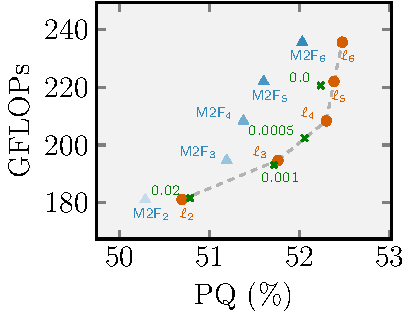
\includegraphics[width=\columnwidth]{figures/images/pareto_plot.pdf}
\end{minipage}%
\begin{minipage}{0.395\textwidth}
\captionof{figure}{\textcolor{map-color}{M2F$_i$} is trained w/ total $i$ layers. \textcolor{r1-color}{$\ell_i$} is result of same model from our Step \stepA. \textcolor{ao(english)}{Values} denote $\beta$. Dataset: COCO.
}
\label{fig:perato}
\end{minipage}
    \end{minipage}%
    \hfill
    \begin{minipage}[!t]{0.495\textwidth}
        \caption{\textbf{Impact of backbone size.} {\ours} shows strong performance \wrt baselines across all backbone sizes on both COCO and Cityscapes datasets while reducing GFLOPs in the transformer encoder. $\dagger$ImageNet-21K pre-trained}
\centering
\resizebox{\columnwidth}{!}{
\begin{tabular}{llccccccc}
\toprule
 && \multicolumn{3}{c}{\textbf{Performance} ($\uparrow$)} && \multicolumn{2}{c}{\textbf{GFLOPs} ($\downarrow$)} \\ \cline{3-5} \cline{7-8}
\multirow{-2}{*}{\textbf{Bakbone}} & \multirow{-2}{*}{\textbf{Model}} & \textbf{PQ} & \textbf{mIOU}$_p$ & \textbf{AP}$_p$ && \textbf{Total} & \textbf{Tx. Enc.} \\ 
\midrule

\multicolumn{8}{c}{\textbf{Dataset}: COCO}\\
\hline
\multirow{2}{*}{\textbf{SWIN-T}} & M2F \cite{cheng2021mask2former} & 52.03 & 62.49 & 42.18 && 235.57  & 121.69\\
& {\ours} & 52.06 & 62.76 & 41.51 && 202.39 & 88.47 \\
\hline
\multirow{2}{*}{\textbf{SWIN-S}} & M2F \cite{cheng2021mask2former} & 54.63 & 64.24 & 44.69 && 316.50 & 121.69 \\
& {\ours} & 54.76 & 64.46 & 44.48 && 275.96 & 81.05 \\
\hline
\multirow{2}{*}{\textbf{SWIN-B}$^\dagger$} & M2F & 56.40 & 67.09  & 46.29 && 470.98 & 122.56 \\
& {\ours} & 56.49 & 66.56 & 46.40 && 425.17 & 76.50 \\
\hline
\multicolumn{8}{c}{\textbf{Dataset}: Cityscapes}\\
\hline
\multirow{2}{*}{\textbf{SWIN-T}} & M2F \cite{cheng2021mask2former} & 64.00 & 80.77 & 39.26 && 537.85 & 281.13 \\
& {\ours} & 64.18 & 80.49 & 39.64 && 507.51  & 250.80 \\

\hline
\multirow{2}{*}{\textbf{SWIN-S}} & M2F \cite{cheng2021mask2former} & 64.84 & 81.76 & 40.73 && 724.29 & 281.13 \\
& {\ours} & 65.12 & 81.64 & 41.17 && 665.38 & 222.22 \\

\hline
\multirow{2}{*}{\textbf{SWIN-B}$^\dagger$} & M2F \cite{cheng2021mask2former} & 66.12 & 82.70 & 42.84 && 1051.19 & 283.14 \\
& {\ours} & 65.44 & 82.05 & 40.51 && 984.73 & 216.69 \\


\bottomrule
\end{tabular}}  
\label{tab:result_backbones}

    \end{minipage}
    \vspace*{-2\baselineskip}
\end{table}
\paragraph{Impact of backbone features.} We analyze the impact of backbone features on \ours in \Tabref{tab:result_backbones} and \Tabref{tab:result_weights}, since our gating network 
 mechanism takes these features as input. 
\begin{itemize}[topsep=0.0em,leftmargin=*]
\setlength\itemsep{0.0em}
    \item \textit{Size variations.} In \tabref{tab:result_backbones}, we evaluate {\ours} with backbones of different sizes. Specifically, we observe the performance with SWIN-Tiny (T), SWIN-Small (S), and SWIN-Base (B) architectures \cite{liu2021swin}. We can observe the adaptability of {\ours} in delivering robust performance efficiency across a range of these backbone sizes. Furthermore, this versatility of {\ours} extends to Lite-M2F meta-architecture as well (see supplementary material).
    %
    \item \textit{Pre-trained weight variations.} We explore how different pre-training strategies for the backbones affect the performance of {\ours} in \tabref{tab:result_weights}. We initialize the backbone weights using both \emph{supervised learning} (SL) and \emph{self-supervised learning} (SSL) techniques on the ImageNet-1K dataset \cite{deng2009imagenet}. For SSL pre-training on the SWIN-T \cite{liu2021swin} backbone, we utilize MoBY \cite{xie2021self}. For SSL pre-training on the Res50 \cite{he2016deep} backbone, we use DINO \cite{caron2021emerging}. With MoBY weights on the SWIN-T backbone, {\ours} maintains 99.7\% of the PQ of M2F while reducing GFLOPs in the transformer encoder by 26.34\%. With DINO weights on the Res50 backbone, we observe a reduction of 29.79\% in GFLOPs in the transformer encoder, alongside a slight improvement in PQ.
\end{itemize}
%
\begin{table}[!t]
    \begin{minipage}{0.495\textwidth}
        \caption{\textbf{Impact on DETR.} We extend our approach to DETR \cite{carion2020end} for object detection tasks as \oursdetr. (Dataset: COCO; Backbone: Res50)}
\centering
\resizebox{\columnwidth}{!}{
\begin{tabular}{lcccccccc}
\toprule
 & \multicolumn{5}{c}{\textbf{Performance} ($\uparrow$)} && \multicolumn{2}{c}{\textbf{GFLOPs} ($\downarrow$)} \\ \cline{2-6} \cline{8-9}
\multirow{-2}{*}{\textbf{Model}} & \textbf{AP} & \textbf{AP}$_{50}$ & \textbf{AP}$_S$ & \textbf{AP}$_M$ & \textbf{AP}$_L$ && \textbf{Total} & \textbf{Tx. Enc.} \\ 
\midrule

DETR \cite{carion2020end} & 42.0 & 62.4 & 20.5 & 45.8 & 61.1 && 83.59 & 9.92 \\
{\oursdetr}($\GPRatio=0.0001$) & 41.9 & 62.2 & 20.8 & 45.8 & 60.4 && 81.87 & 6.41 \\
{\oursdetr}($\GPRatio=0.001$) & 40.9 & 61.5 & 20.2 & 44.5 & 59.1 && 79.92 & 4.52 \\
{\oursdetr}($\GPRatio=0.01$) & 40.2 & 61.0 & 18.7 & 43.6 & 58.8 && 79.33 & 3.94 \\

\bottomrule
\end{tabular}}  
\label{tab:result_detr}
    \end{minipage}%
    \hfill
    \begin{minipage}{0.495\textwidth}
        \caption{\textbf{Impact of backbone weights.} {\ours} applies to backbone weights obtained through self-supervised pre-training as well. (Dataset: COCO)}
\centering
\resizebox{\columnwidth}{!}{
\begin{tabular}{llcccccccc}
\toprule
 && \multicolumn{3}{c}{\textbf{Performance} ($\uparrow$)} && \multicolumn{2}{c}{\textbf{GFLOPs} ($\downarrow$)} \\ \cline{3-5} \cline{7-8}
\multirow{-2}{*}{\textbf{Bakbone}} & \multirow{-2}{*}{\textbf{Model}} & \textbf{PQ} & \textbf{mIOU}$_p$ & \textbf{AP}$_p$ && \textbf{Total} & \textbf{Tx. Enc.} \\ 
\midrule
\multirow{2}{*}{\textbf{SWIN-T(MoBY\cite{xie2021moby})}} & M2F\cite{cheng2021mask2former}  & 51.64 & 62.42 & 41.93 && 235.57 & 121.69 \\
& {\ours} & 51.48 & 62.49  & 41.27 && 203.56 & 89.64 \\
\hline
\multirow{2}{*}{\textbf{Res50(DINO\cite{caron2021emerging})}} & M2F\cite{cheng2021mask2former} & 51.57 & 61.65 & 41.24 && 229.41 & 126.05 \\
& {\ours} & 51.89 & 61.67 & 41.30 && 191.97 & 88.50 \\
\bottomrule
\end{tabular}}  
\label{tab:result_weights}
    \end{minipage}
\end{table}
\paragraph{Performance in object detection.} To demonstrate the applicability of our method beyond segmentation, we extend our proposed three step recipe for object detection task using DETR \cite{carion2020end} for object detection task and name it \oursdetr. In particular, we vary the values of the adaptation factor $\GPRatio$ to analyze performance-computation trade-offs of \oursdetr in \tabref{tab:result_detr}. Clearly, the resultant architecture maintains the performance but helps in reducing the computations of the encoder (\eg, it achieves a 35.38\% reduction in GFLOPs in the transformer encoder without significantly impacting performance).

\subsection{Qualitative Comparisons}
\begin{figure}[!ht]
\begin{tcbraster}[enhanced,
    blank, 
    raster columns=3,
    raster equal height,
    ]
    \tcbincludegraphics[]{figures/qual_result_images/coco/exp10/000000297427.jpg}
    \tcbincludegraphics[]{figures/qual_result_images/coco/exp10/000000297427_m2f.jpg}
    \tcbincludegraphics[flip title={boxsep=0.75mm}]{figures/qual_result_images/coco/exp10/000000297427_ours.jpg}
    \vspace*{-2\baselineskip}
    %
    \tcbincludegraphics[]{figures/qual_result_images/coco/exp11/000000300913.jpg}
    \tcbincludegraphics[]{figures/qual_result_images/coco/exp11/000000300913_m2f.jpg}
    \tcbincludegraphics[flip title={boxsep=0.75mm}]{figures/qual_result_images/coco/exp11/000000300913_ours.jpg}
    \vspace*{-3\baselineskip}
    %
    \tcbincludegraphics[]{figures/qual_result_images/cityscapes/exp1/frankfurt_000000_016286_leftImg8bit.png}
    \tcbincludegraphics[]{figures/qual_result_images/cityscapes/exp1/frankfurt_000000_016286_leftImg8bit_m2f.png}
    \tcbincludegraphics[flip title={boxsep=0.75mm}]{figures/qual_result_images/cityscapes/exp1/frankfurt_000000_016286_leftImg8bit_ours.png}
    \vspace*{-6.25\baselineskip}
    %
    \tcbincludegraphics[]{figures/qual_result_images/cityscapes/exp2/frankfurt_000001_004327_leftImg8bit.png}
    \tcbincludegraphics[]{figures/qual_result_images/cityscapes/exp2/frankfurt_000001_004327_leftImg8bit_m2f.png}
    \tcbincludegraphics[flip title={boxsep=0.75mm}]{figures/qual_result_images/cityscapes/exp2/frankfurt_000001_004327_leftImg8bit_ours.png}
    \vspace*{-2\baselineskip}
   \end{tcbraster} 
    \caption{\textbf{Qualitative visualizations.} We illustrate few examples of predicted segmentation maps from M2F \cite{cheng2021mask2former} (\textit{middle} column) and \ours (\textit{last} column). \textit{Top} two rows are from the COCO dataset, whereas \textit{bottom} two rows are from the Cityscapes dataset. (Backbone: Swin-T) \textit{Zoom-in for best view}.}
    \label{fig:qual_result}
\end{figure}
We present a few examples of predicted segmentation maps in \Figref{fig:qual_result} with SWIN-T \cite{liu2021swin} backbone. Compared to the parent architecture, \ours consistently shows strong performance while self-selecting the encoder layers based on the input examples, both in everyday scenes (on COCO dataset) as well as intricate traffic scenes (on Cityscapes dataset).